\section{实验结果}
\label{sec:ink-results}

\subsection{跨骨干与任务规模汇总}

\begin{table}[!htbp]
  \centering
  \caption{视觉模型合并汇总：三个骨干分别预留 8、14、20 tasks。单元格为平均绝对准确率$_{(\text{归一化准确率})}$（\%）；-- 表示本地缺少可核验结果。}
  \label{tab:ink-vision-summary}
  \setlength{\tabcolsep}{3.0pt}
  \renewcommand{\arraystretch}{1.15}
  \resizebox{\textwidth}{!}{%
  \begin{tabular}{@{}lccc|ccc|ccc@{}}
    \toprule
    \multirow{2}{*}{\textbf{Method}} &
    \multicolumn{3}{c}{\texttt{ViT-B-32}} &
    \multicolumn{3}{c}{\texttt{ViT-B-16}} &
    \multicolumn{3}{c}{\texttt{ViT-L-14}} \\
    \cmidrule(lr){2-4}\cmidrule(lr){5-7}\cmidrule(l){8-10}
    & 8 tasks & 14 tasks & 20 tasks & 8 tasks & 14 tasks & 20 tasks & 8 tasks & 14 tasks & 20 tasks \\
    \midrule
    Individual FT & $89.93_{(100.00)}$ & \placeholdervalue{--} & \placeholdervalue{--} & \placeholdervalue{--} & \placeholdervalue{--} & \placeholdervalue{--} & \placeholdervalue{--} & \placeholdervalue{--} & \placeholdervalue{--} \\
    \midrule
    Zero-shot & $46.69_{(53.63)}$ & \placeholdervalue{--} & \placeholdervalue{--} & \placeholdervalue{--} & \placeholdervalue{--} & \placeholdervalue{--} & \placeholdervalue{--} & \placeholdervalue{--} & \placeholdervalue{--} \\
    Weight Avg. & $66.42_{(73.83)}$ & \placeholdervalue{--} & \placeholdervalue{--} & \placeholdervalue{--} & \placeholdervalue{--} & \placeholdervalue{--} & \placeholdervalue{--} & \placeholdervalue{--} & \placeholdervalue{--} \\
    Task Arith. & $66.49_{(73.76)}$ & \placeholdervalue{--} & \placeholdervalue{--} & \placeholdervalue{--} & \placeholdervalue{--} & \placeholdervalue{--} & \placeholdervalue{--} & \placeholdervalue{--} & \placeholdervalue{--} \\
    TIES & $69.41_{(76.94)}$ & \placeholdervalue{--} & \placeholdervalue{--} & \placeholdervalue{--} & \placeholdervalue{--} & \placeholdervalue{--} & \placeholdervalue{--} & \placeholdervalue{--} & \placeholdervalue{--} \\
    Consensus TA & $70.36_{(77.86)}$ & \placeholdervalue{--} & \placeholdervalue{--} & \placeholdervalue{--} & \placeholdervalue{--} & \placeholdervalue{--} & \placeholdervalue{--} & \placeholdervalue{--} & \placeholdervalue{--} \\
    Iso-C & $81.33_{(90.21)}$ & \placeholdervalue{--} & \placeholdervalue{--} & \placeholdervalue{--} & \placeholdervalue{--} & \placeholdervalue{--} & \placeholdervalue{--} & \placeholdervalue{--} & \placeholdervalue{--} \\
    Iso-CTS & $81.04_{(89.86)}$ & \placeholdervalue{--} & \placeholdervalue{--} & \placeholdervalue{--} & \placeholdervalue{--} & \placeholdervalue{--} & \placeholdervalue{--} & \placeholdervalue{--} & \placeholdervalue{--} \\
    TSV-M & $81.35_{(90.08)}$ & \placeholdervalue{--} & \placeholdervalue{--} & \placeholdervalue{--} & \placeholdervalue{--} & \placeholdervalue{--} & \placeholdervalue{--} & \placeholdervalue{--} & \placeholdervalue{--} \\
    RegMean & $81.27_{(90.00)}$ & \placeholdervalue{--} & \placeholdervalue{--} & \placeholdervalue{--} & \placeholdervalue{--} & \placeholdervalue{--} & \placeholdervalue{--} & \placeholdervalue{--} & \placeholdervalue{--} \\
    WUDI & $82.55_{(91.37)}$ & \placeholdervalue{--} & \placeholdervalue{--} & \placeholdervalue{--} & \placeholdervalue{--} & \placeholdervalue{--} & \placeholdervalue{--} & \placeholdervalue{--} & \placeholdervalue{--} \\
    LiNeS (Iso-C) & $83.37_{(92.58)}$ & \placeholdervalue{--} & \placeholdervalue{--} & \placeholdervalue{--} & \placeholdervalue{--} & \placeholdervalue{--} & \placeholdervalue{--} & \placeholdervalue{--} & \placeholdervalue{--} \\
    CoM & $83.38_{(92.29)}$ & \placeholdervalue{--} & \placeholdervalue{--} & \placeholdervalue{--} & \placeholdervalue{--} & \placeholdervalue{--} & \placeholdervalue{--} & \placeholdervalue{--} & \placeholdervalue{--} \\
    ESM & $84.19_{(93.48)}$ & \placeholdervalue{--} & \placeholdervalue{--} & \placeholdervalue{--} & \placeholdervalue{--} & \placeholdervalue{--} & \placeholdervalue{--} & \placeholdervalue{--} & \placeholdervalue{--} \\
    SVC (Iso-CTS) & $81.61_{(90.79)}$ & \placeholdervalue{--} & \placeholdervalue{--} & \placeholdervalue{--} & \placeholdervalue{--} & \placeholdervalue{--} & \placeholdervalue{--} & \placeholdervalue{--} & \placeholdervalue{--} \\
    SVC (ESM) & $82.38_{(91.58)}$ & \placeholdervalue{--} & \placeholdervalue{--} & \placeholdervalue{--} & \placeholdervalue{--} & \placeholdervalue{--} & \placeholdervalue{--} & \placeholdervalue{--} & \placeholdervalue{--} \\
    \rowcolor{black!8}
    \textbf{\method{}} & $\boldsymbol{86.95_{(96.54)}}$ & \placeholdervalue{--} & \placeholdervalue{--} & \placeholdervalue{--} & \placeholdervalue{--} & \placeholdervalue{--} & \placeholdervalue{--} & \placeholdervalue{--} & \placeholdervalue{--} \\
    \bottomrule
  \end{tabular}%
  }
\end{table}


表~\ref{tab:ink-vision-summary} 将三个视觉骨干及三种任务规模合并为一张主表。ViT-B/32 的 8 tasks 一列保留已有复现记录，其他单元格为待补位置，不据此作规模扩展结论。

当前种子 0 的 \method{} 平均绝对准确率为 $86.95\%$，相对独立专家的归一化准确率为 $96.54\%$。其绝对准确率比 ESM、CoM 和 RegMean 分别高 $2.76$、$3.57$ 和 $5.67$ 个百分点，与 Individual FT 专家参考的差距为 $2.99$ 个百分点。

\FloatBarrier
\subsection{Flan-T5-base 持续模型合并}

\begin{table}[!htbp]
  \centering
  \caption{Flan-T5-base 八任务持续合并结果版式预留。所有灰色数字（含 $\pm$ 项）均为随机占位，非实测均值或标准差。}
  \label{tab:ink-t5-results}
  \setlength{\tabcolsep}{3.0pt}
  \renewcommand{\arraystretch}{1.18}
  \resizebox{\textwidth}{!}{%
  \begin{tabular}{@{}lrrrrrrrr|c@{}}
    \toprule
    \textbf{Method} & CoLA & MNLI & MRPC & QNLI & QQP & RTE & SST2 & STSB & ACC($\uparrow$) \\
    \midrule
    (Ref.) Single Fine-Tune & \placeholdervalue{71.8} & \placeholdervalue{90.9} & \placeholdervalue{67.1} & \placeholdervalue{83.1} & \placeholdervalue{82.8} & \placeholdervalue{81.0} & \placeholdervalue{91.1} & \placeholdervalue{85.6} & \placeholdervalue{$81.7\pm 1.3$} \\
    \midrule
    Zero-shot & \placeholdervalue{81.4} & \placeholdervalue{77.8} & \placeholdervalue{69.6} & \placeholdervalue{70.7} & \placeholdervalue{70.7} & \placeholdervalue{66.3} & \placeholdervalue{89.2} & \placeholdervalue{83.9} & \placeholdervalue{$76.2\pm 0.7$} \\
    Weight Avg. & \placeholdervalue{77.0} & \placeholdervalue{72.9} & \placeholdervalue{71.4} & \placeholdervalue{84.7} & \placeholdervalue{86.9} & \placeholdervalue{88.7} & \placeholdervalue{90.1} & \placeholdervalue{70.1} & \placeholdervalue{$80.2\pm 0.4$} \\
    Task Arith. & \placeholdervalue{92.0} & \placeholdervalue{73.0} & \placeholdervalue{71.0} & \placeholdervalue{72.1} & \placeholdervalue{73.2} & \placeholdervalue{67.4} & \placeholdervalue{87.4} & \placeholdervalue{80.1} & \placeholdervalue{$77.0\pm 0.7$} \\
    TIES & \placeholdervalue{75.0} & \placeholdervalue{74.0} & \placeholdervalue{73.8} & \placeholdervalue{67.4} & \placeholdervalue{66.4} & \placeholdervalue{72.4} & \placeholdervalue{81.2} & \placeholdervalue{65.7} & \placeholdervalue{$72.0\pm 0.2$} \\
    Consensus TA & \placeholdervalue{82.6} & \placeholdervalue{89.4} & \placeholdervalue{70.0} & \placeholdervalue{83.2} & \placeholdervalue{71.5} & \placeholdervalue{89.4} & \placeholdervalue{87.3} & \placeholdervalue{78.0} & \placeholdervalue{$81.4\pm 0.2$} \\
    Iso-C & \placeholdervalue{83.2} & \placeholdervalue{78.0} & \placeholdervalue{82.7} & \placeholdervalue{71.0} & \placeholdervalue{75.5} & \placeholdervalue{80.3} & \placeholdervalue{92.3} & \placeholdervalue{81.3} & \placeholdervalue{$80.5\pm 0.4$} \\
    Iso-CTS & \placeholdervalue{80.8} & \placeholdervalue{68.7} & \placeholdervalue{86.5} & \placeholdervalue{65.3} & \placeholdervalue{82.8} & \placeholdervalue{83.6} & \placeholdervalue{90.4} & \placeholdervalue{92.1} & \placeholdervalue{$81.3\pm 0.5$} \\
    TSV-M & \placeholdervalue{81.2} & \placeholdervalue{66.9} & \placeholdervalue{71.9} & \placeholdervalue{75.0} & \placeholdervalue{86.5} & \placeholdervalue{82.8} & \placeholdervalue{69.5} & \placeholdervalue{74.0} & \placeholdervalue{$76.0\pm 0.6$} \\
    RegMean & \placeholdervalue{82.2} & \placeholdervalue{72.4} & \placeholdervalue{68.2} & \placeholdervalue{89.2} & \placeholdervalue{91.6} & \placeholdervalue{88.2} & \placeholdervalue{92.8} & \placeholdervalue{74.7} & \placeholdervalue{$82.4\pm 0.1$} \\
    WUDI & \placeholdervalue{80.7} & \placeholdervalue{83.1} & \placeholdervalue{83.8} & \placeholdervalue{80.9} & \placeholdervalue{92.8} & \placeholdervalue{89.6} & \placeholdervalue{67.0} & \placeholdervalue{79.8} & \placeholdervalue{$82.2\pm 0.8$} \\
    LiNeS (Iso-C) & \placeholdervalue{87.3} & \placeholdervalue{77.9} & \placeholdervalue{68.1} & \placeholdervalue{67.3} & \placeholdervalue{67.0} & \placeholdervalue{74.1} & \placeholdervalue{66.9} & \placeholdervalue{76.1} & \placeholdervalue{$73.1\pm 0.5$} \\
    CoM & \placeholdervalue{70.2} & \placeholdervalue{65.6} & \placeholdervalue{88.4} & \placeholdervalue{65.0} & \placeholdervalue{91.9} & \placeholdervalue{87.4} & \placeholdervalue{82.1} & \placeholdervalue{74.0} & \placeholdervalue{$78.1\pm 1.4$} \\
    ESM & \placeholdervalue{82.5} & \placeholdervalue{92.2} & \placeholdervalue{91.0} & \placeholdervalue{84.8} & \placeholdervalue{76.2} & \placeholdervalue{84.6} & \placeholdervalue{77.0} & \placeholdervalue{66.9} & \placeholdervalue{$81.9\pm 0.2$} \\
    SVC (Iso-CTS) & \placeholdervalue{76.7} & \placeholdervalue{84.5} & \placeholdervalue{74.6} & \placeholdervalue{72.0} & \placeholdervalue{73.2} & \placeholdervalue{76.1} & \placeholdervalue{86.9} & \placeholdervalue{75.9} & \placeholdervalue{$77.5\pm 0.3$} \\
    SVC (ESM) & \placeholdervalue{86.5} & \placeholdervalue{76.6} & \placeholdervalue{92.2} & \placeholdervalue{89.9} & \placeholdervalue{65.7} & \placeholdervalue{83.6} & \placeholdervalue{90.8} & \placeholdervalue{70.6} & \placeholdervalue{$82.0\pm 1.2$} \\
    \rowcolor{black!8}
    \textbf{\method{} (Ours)} & \placeholdervalue{65.6} & \placeholdervalue{91.5} & \placeholdervalue{82.6} & \placeholdervalue{83.4} & \placeholdervalue{74.9} & \placeholdervalue{83.1} & \placeholdervalue{69.0} & \placeholdervalue{65.7} & \placeholdervalue{$77.0\pm 0.1$} \\
    \bottomrule
  \end{tabular}%
  }
  \par\smallskip
  {\footnotesize 随机占位 / 非实验结果。方法列表补齐视觉表基线；不沿用视觉结果。各方法的 T5 适配与持续合并实现、任务顺序、重复次数及 ACC 统计口径待核验。}
\end{table}


表~\ref{tab:ink-t5-results} 按参考表预留 Flan-T5-base 在八个任务上持续合并后的结果，并补齐视觉表中的方法列表。独立微调参考行置于顶部，Zero-shot 与各合并基线居中，\method{} 行以灰底突出。方法名称统一不表示其 T5 适配或持续合并版本已实现，也不沿用视觉实验的数值。所有数字及 $\pm$ 项均为排版占位，不代表已完成的运行、随机种子均值或标准差。正式实验记录补齐后，再按确认的任务顺序与指标协议填写 ACC 和逐任务表现。

\FloatBarrier
\subsection{种子复核}

逐任务明细见附录~\ref{apdx:ink-vitb32-details} 的表~\ref{tab:ink-vitb32-results}。

留出集轨迹与选择协议一致：种子 0 从轮次 0 的平均教师 KL $0.33332061$ 降至所选轮次 3 的 $0.15524809$，第 4 轮所有块步长均为零并停止。独立校准种子 1 在相同冻结配置下选择轮次 4，平均准确率为 $87.0496\%$，对应留出教师 KL 为 $0.13468810$。两个种子的平均准确率为 $86.9974\%$，总体标准差为 $0.0522$ 个百分点。该复核只衡量两次独立校准抽样下的稳定性，不替代更大规模的多种子评估。
\FloatBarrier

\subsection{输出几何收缩：稳定性与方向信息（待验证）}
\label{sec:ink-parameter-analysis}

以下三节将原参数图拆为独立分析。所有曲线均为\textbf{预期趋势示意，不是实验结果}；纵轴不提供准确率或 KL 数值，也不绘制虚构误差带。实际结果可能与这些假设不同。

\paragraph{要做什么。}
只扫描输出几何收缩强度，其余设置保持冻结协议不变。对非零输出二阶矩，先沿用实现的平均对角归一化得到 $\bar G$，再使用
\[
  G_\alpha=(1-\alpha)\bar G+\alpha I,\qquad
  \alpha\in\{0,0.1,\ldots,1.0\}.
\]
$\alpha=0$ 保留原方向结构，$\alpha=1$ 将非零输出度量变为单位矩阵；原始全零统计仍保持为零。输入几何不变更其收缩规则。现有逐任务、逐层自动收缩作为另一个完整配置单独运行，而不是人为对应到一个固定 $\alpha$。

\begin{figure}[!htbp]
  \centering
  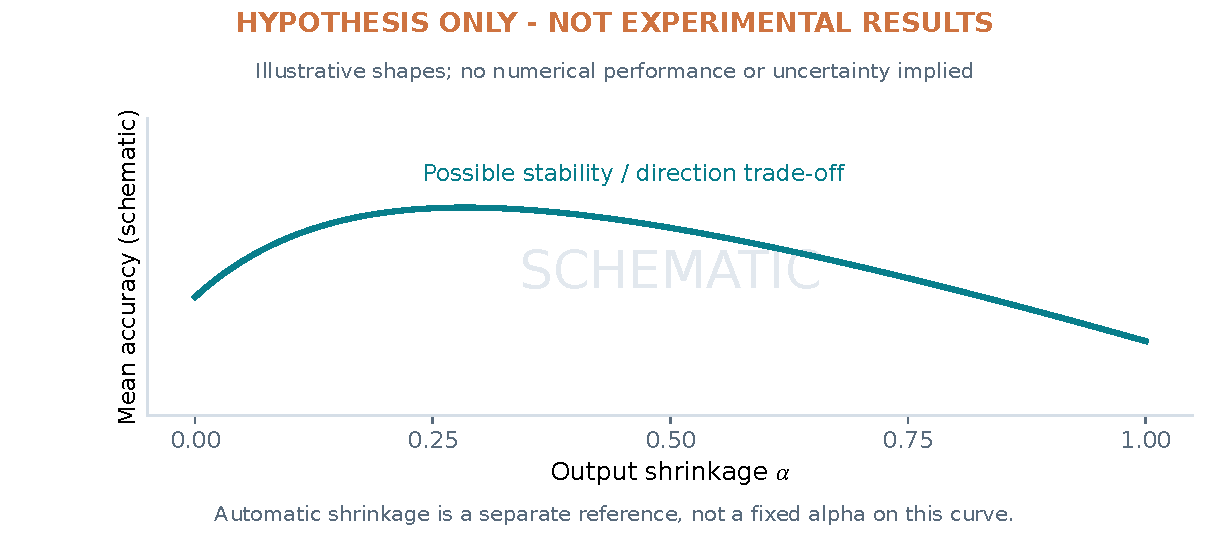
\includegraphics[width=0.78\linewidth]{figures/hypothesis_shrinkage.pdf}
  \caption{\textbf{输出收缩的预期趋势示意，非实验结果。}假设适度收缩能稳定有限样本的几何估计，而过强收缩会削弱方向信息；曲线可能存在宽缓的较优区间，但其形状和位置均待验证。纵轴无实测准确率刻度，自动收缩参照尚未绘制。}
  \label{fig:ink-parameter-analysis}
\end{figure}


\paragraph{如何解读。}
我们希望检验：轻度收缩是否有助于稳定有限样本估计，而强收缩是否丢失有用的输出方向信息。图~\ref{fig:ink-parameter-analysis} 画出一种可能的先升后降趋势，不是对最优 $\alpha$ 的预测。如果曲线平坦，就说明在该协议下对收缩不敏感；若单位度量不差，则不能据此声称输出方向信息不可替代。仅凭收缩曲线也不能分离方向结构和数值条件的全部影响。

\FloatBarrier
\subsection{统计样本量：多少无标签数据才够用（待验证）}
\label{sec:ink-sample-size-analysis}

\paragraph{要做什么。}
比较完整方法与每轮重估的当前模型 Fisher 对照。每个校准种子先固定统计样本顺序，再取前 32、64、128、256 个构成嵌套子集；两种方法在每个样本量下使用完全相同的子集。留出集始终是另外同一组 256 个样本，不能随着统计样本量缩小，也不能与统计子集重叠。每个设置从相同初始化独立运行完整合并流程，不能沿用上一个样本量的已合并权重。除样本量和输出几何类型外，求解预算、自动收缩规则、步长选择及轮次上限均相同。

\begin{figure}[!htbp]
  \centering
  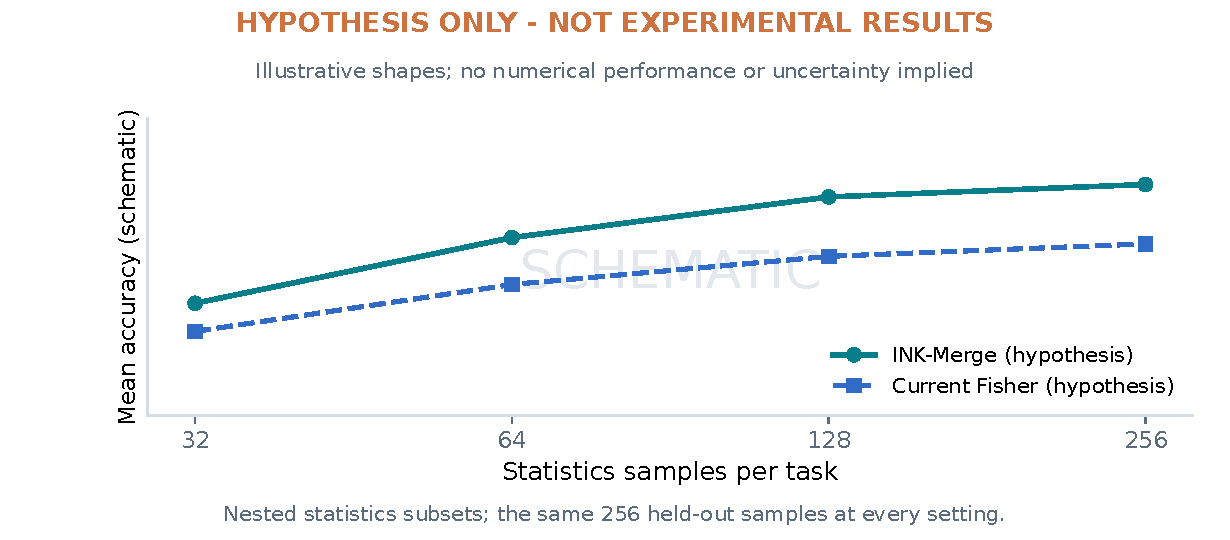
\includegraphics[width=0.78\linewidth]{figures/hypothesis_samples.pdf}
  \caption{\textbf{统计样本量的预期趋势示意，非实验结果。}待验证假设是样本增加带来收益递减，修正几何可能在有限样本下优于当前 Fisher。曲线间距和拐点仅供解释，既不是测得的性能差值，也不证明 128 或 256 个样本已经足够。}
  \label{fig:ink-sample-size-analysis}
\end{figure}


\paragraph{如何解读。}
图~\ref{fig:ink-sample-size-analysis} 示意的假设是：样本更多时估计更稳定，平均准确率逐渐提高并趋于饱和；修正几何可能在小样本区间更有效。需要用真实数据判断曲线是否饱和、两种方法的差异是否跨种子一致，不能从示意图认定某个样本数已足够。横轴只计统计样本，实际无标签数据预算还包括固定的 256 个留出样本；512 或 1024 个统计样本需另备数据，不能从留出集挪用。

\FloatBarrier
\subsection{迭代重估：动态输出几何是否必要（待验证）}
\label{sec:ink-iteration-analysis}

\paragraph{要做什么。}
从同一初始化分别运行三组对照：每轮重估当前模型 Fisher；固定初始输出修正几何 $G^{(0)}$、但持续重估输入几何 $A$；完整方法同时重估 $A,G$。在每个变体各自的轨迹上记录第 0--4 轮状态，并用同一独立诊断集计算八任务等权平均教师 KL。该诊断集不得参与几何估计、步长或轮次选择；所有对照使用相同统计和留出划分。现有固定首轮统计开关会同时冻结 $A,G$，不能直接用来实现第二组对照。

\begin{figure}[!htbp]
  \centering
  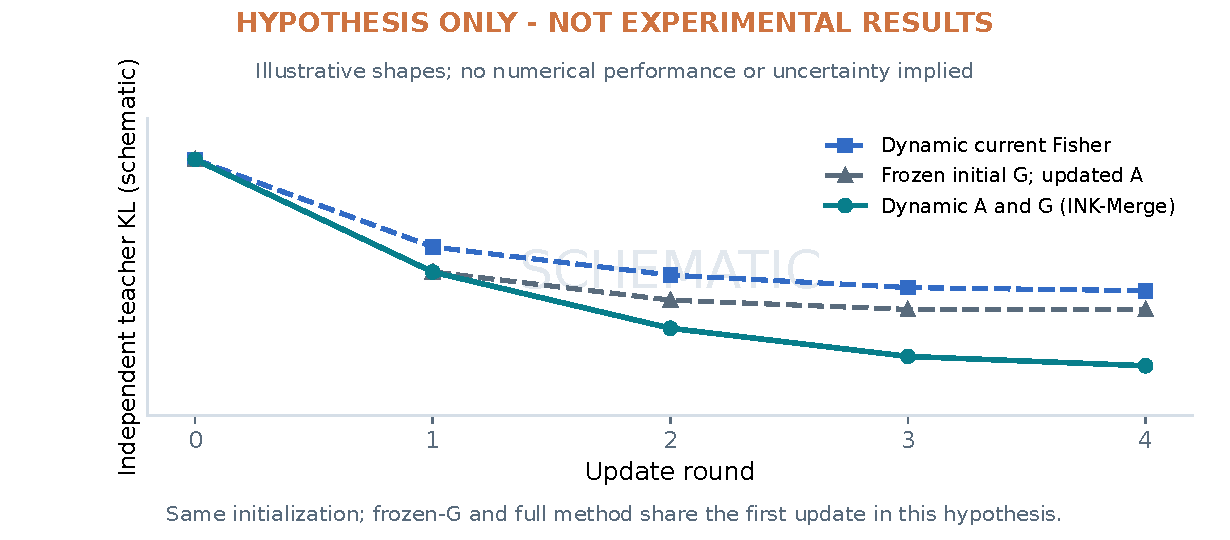
\includegraphics[width=0.78\linewidth]{figures/hypothesis_rounds.pdf}
  \caption{\textbf{动态性对照的预期趋势示意，非实验结果。}三种设置共享初始化；仅冻结初始 $G$ 与完整方法在相同协议下共享第一轮候选更新，差异应在后续重估中体现。图示假设动态修正几何可继续降低独立 KL，不表示真实曲线必然单调或方法排名已确定。}
  \label{fig:ink-iteration-analysis}
\end{figure}


\paragraph{如何解读。}
图~\ref{fig:ink-iteration-analysis} 中仅冻结 $G$ 与完整方法的首轮更新重合：此时两者都使用相同的初始几何。后续若完整方法持续优于冻结 $G$，才支持重估输出几何的价值；若优于动态 Fisher，才支持残差条件化在该设置下的价值。独立 KL 可能回升，不要求单调下降。提前停止时只报告已完成轮次，或将保持不变的尾段明确标注为停止后的状态延续，不伪装成新更新。

\paragraph{共同评估约束。}
上述扫描固定使用校准种子 0、1、2；真实结果分别保存每种子的曲线，再报告均值与样本标准差。当前仅有两个种子的冻结记录，不足以补齐这些实验。所有配置、数据划分和扫描点在运行前固定；测试准确率只用于最终诊断报告，不用于反选默认参数、轮次或步长。既有留出 KL 轨迹仅说明选择过程，不能替代独立诊断。前面的图~\ref{fig:ink-motivation} 仍单独负责修正能量的机制诊断。

\FloatBarrier
\subsection{核心设计消融（待运行）}
\label{sec:ink-core-ablation}

\begin{table}[!htbp]
  \centering
  \caption{核心设计消融表位。\textbf{全部待运行}；-- 表示缺少同协议实验结果，完整方法也需在相同的新种子协议下运行，不将现有两种子结果拼入本表。}
  \label{tab:ink-core-ablation}
  \small
  \setlength{\tabcolsep}{4pt}
  \renewcommand{\arraystretch}{1.35}
  \begin{tabularx}{\linewidth}{@{}X X cc@{}}
    \toprule
    对照 & 验证问题 & 平均准确率 $\uparrow$ & 诊断 KL $\downarrow$ \\
    \midrule
    \rowcolor{black!8}
    完整 \method{} & 同协议参考 & -- & -- \\
    当前 Fisher 替换修正 $G$ & 残差条件化 & -- & -- \\
    仅固定 $G^{(0)}$，更新 $A$ & 动态输出几何 & -- & -- \\
    去掉 Pearson 归一化 & 样本尺度控制 & -- & -- \\
    仅做全局线搜索 & 逐块步长选择 & -- & -- \\
    每轮完整采用候选更新 & 保守更新 & -- & -- \\
    \bottomrule
  \end{tabularx}
\end{table}


表~\ref{tab:ink-core-ablation} 预留六组对照，各组保持统计样本、留出样本、初始化、求解预算与收缩规则可比，未来报告至少三个相同校准种子下的均值与标准差。仅全局线搜索的变体关闭逐块精调；完整候选更新的变体则每轮直接接受候选权重，不依据留出 KL 拒绝该轮更新。后者需要专门实现并验证，不能把要求包含零的现有步长候选接口简单设成 $\{1\}$。所有新变体结果目前均为空，未改变正文已有的冻结实验结论。

单轮 0--1 步长诊断、初始化依赖和求解成本图位分别见附录~\ref{apdx:ink-step-size}、\ref{apdx:ink-initialization}、\ref{apdx:ink-cost}。若计算预算有限，优先级为核心消融表、输出收缩扫描、统计样本量扫描。
\FloatBarrier
